\section{Figures}
\label{sec:figures}

\begin{figure}[ht]
	\centering
	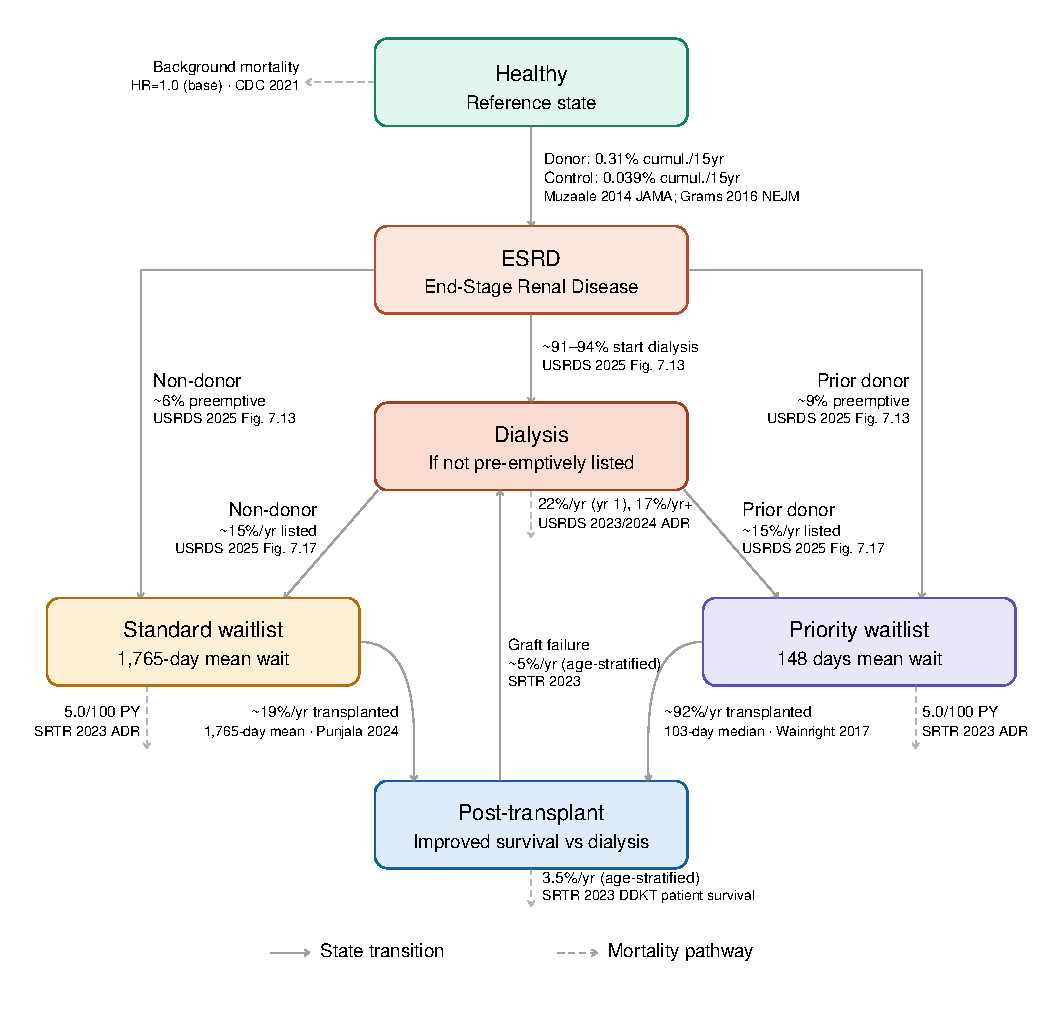
\includegraphics[width=\linewidth]{figures/markov_model_kidney_donation.pdf}
	\caption{Markov state-transition model for kidney donation. Boxes represent the seven mutually exclusive health states; arrows show permitted transitions. The donor arm (upper pathway) routes ESRD-onset patients to the Priority waitlist; the non-donor arm routes to the Standard waitlist. The Dead state is absorbing.}
	\label{fig:markov}
\end{figure}

\begin{figure}[ht]
	\centering
	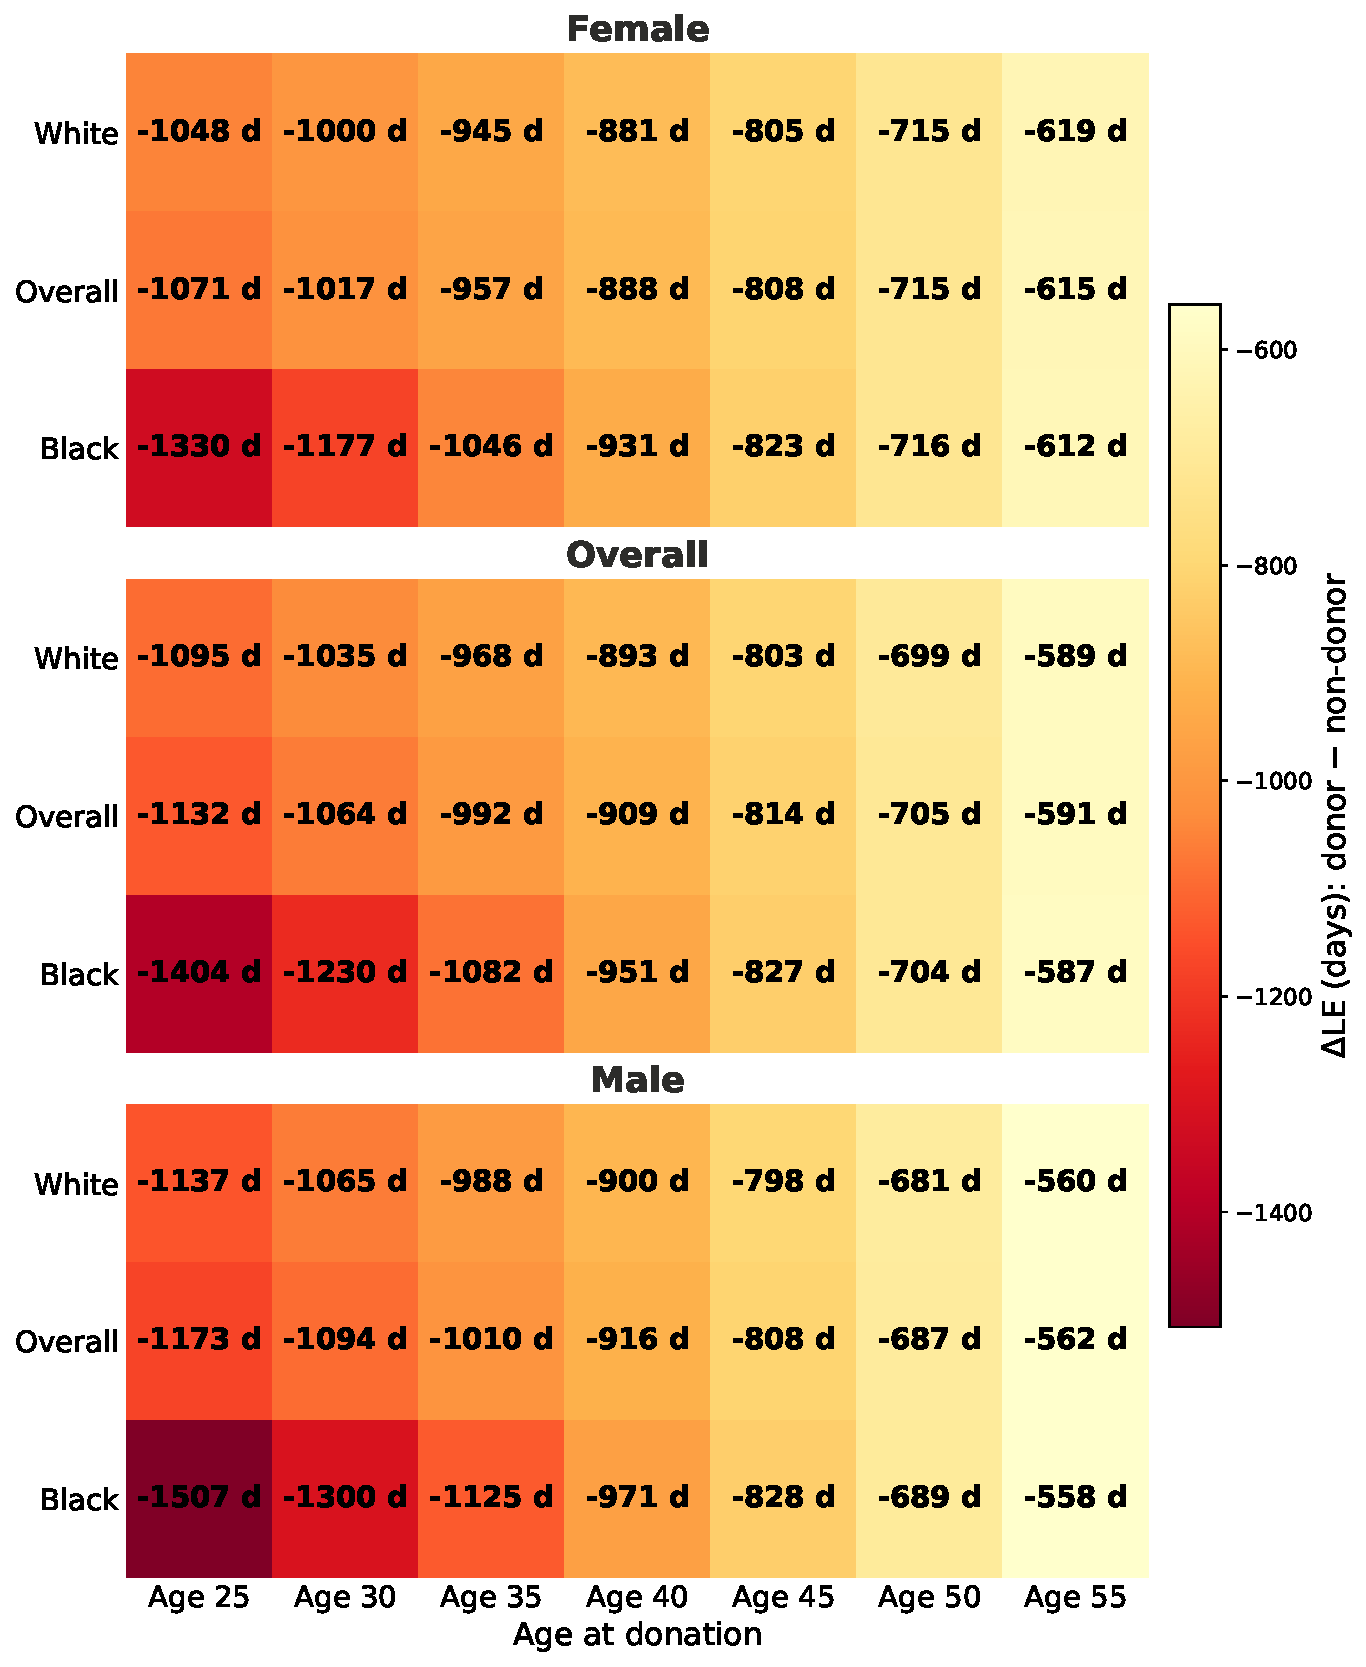
\includegraphics[width=\linewidth]{figures/kidney_model_age_race_sex_matrix.pdf}
	\caption{\textbf{Life-expectancy impact of kidney donation by age, race, and sex.} Each cell shows $\Delta\text{LE}$ (donor minus non-donor, days) for the indicated sex panel, race row, and age-at-donation column. Age at donation dominates: a Black male donor at age~25 loses 1{,}507~days, compared with 619~days for a White female donor at age~55. At age~25, the largest within-age contrast (Black male vs.\ White female) is 1{,}507 vs.\ 1{,}048~days, respectively, a 44\% difference.}
	\label{fig:age_race_sex_matrix}
\end{figure}

\begin{figure}[ht]
	\centering
	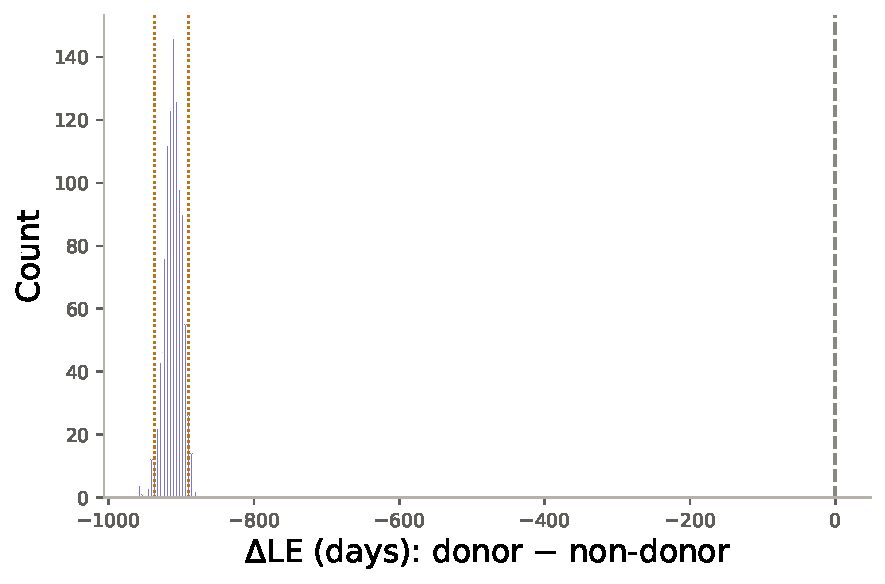
\includegraphics[width=\linewidth]{figures/kidney_model_B_psa.pdf}
	\caption{\textbf{Probabilistic sensitivity analysis (PSA).} Histogram of $\Delta\text{LE}$ (donor minus non-donor, days). The dashed vertical line marks zero; orange dotted lines mark the 95\% credible interval bounds.}
	\label{fig:psa}
\end{figure}

\begin{figure}[ht]
	\centering
	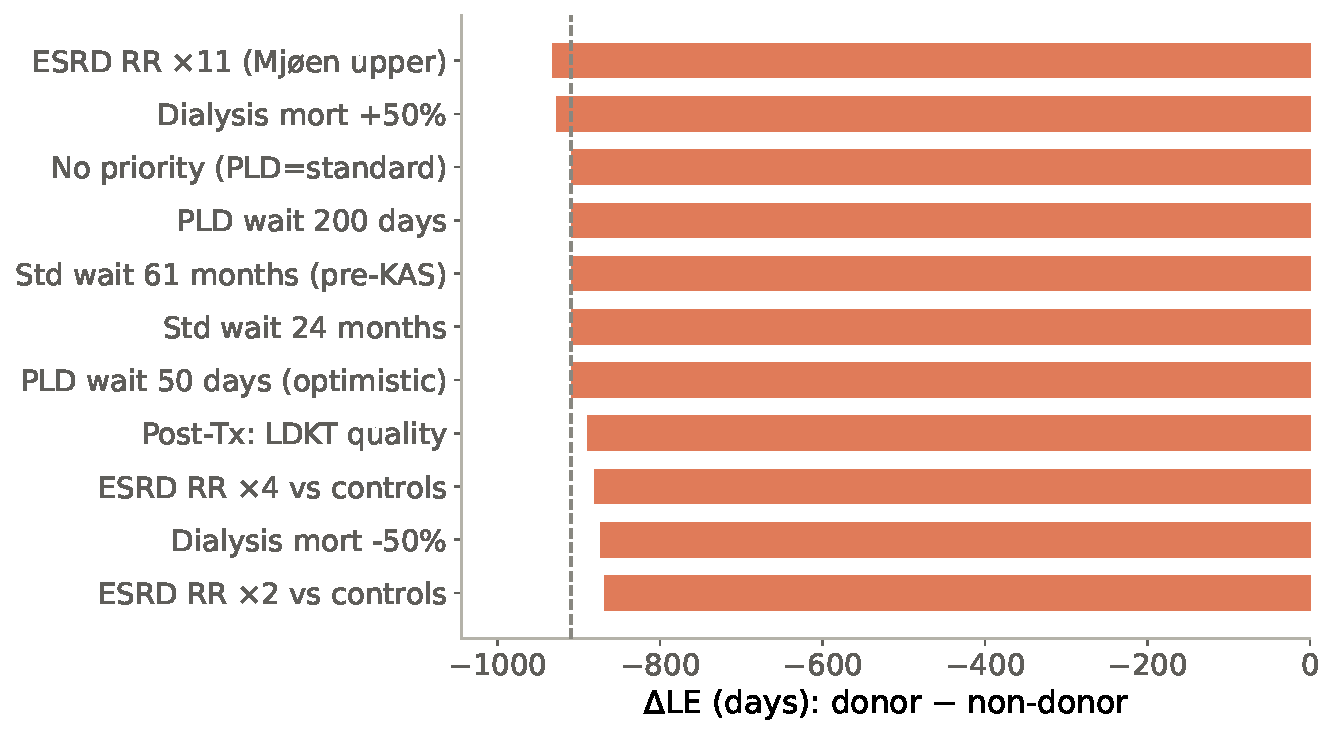
\includegraphics[width=\linewidth]{figures/kidney_model_C_tornado.pdf}
	\caption{\textbf{One-way sensitivity analysis: tornado chart.} Each bar shows the $\Delta\text{LE}$ resulting from testing the indicated parameter value, holding the donor all-cause mortality HR fixed at its base-case time-varying profile (see Table~\ref{tab:owsa} for exact values; Figure~\ref{fig:hr_scenarios} for sensitivity to the HR assumption itself). Vertical dashed line shows base case. With the HR held fixed, no parameter shifts $\Delta\text{LE}$ by more than 42~days; priority waitlist parameters (``No priority'' and ``PLD wait'' rows) are barely distinguishable from base case, confirming the negligible population-level effect of transplant priority.}
	\label{fig:tornado}
\end{figure}

\begin{figure}[ht]
	\centering
	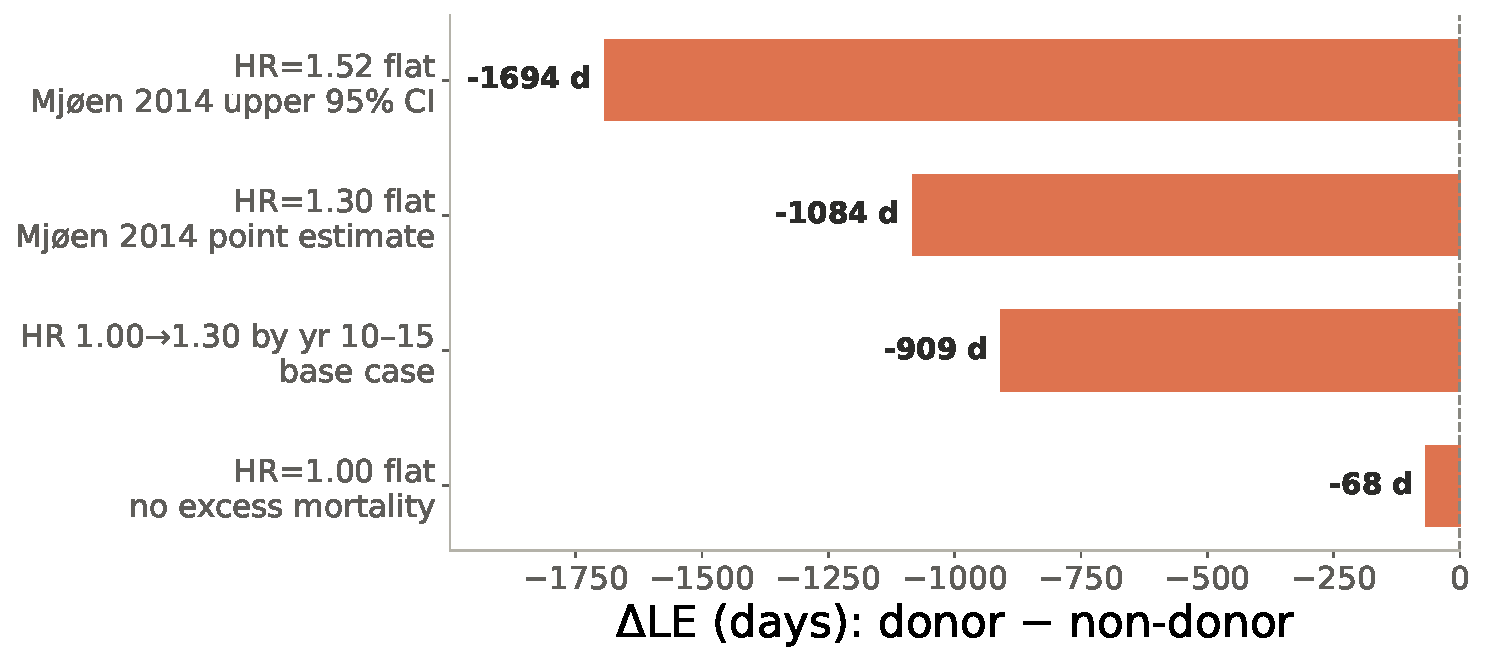
\includegraphics[width=\linewidth]{figures/kidney_model_F_hr_scenarios.pdf}
	\caption{\textbf{Structural sensitivity to the donor all-cause mortality HR.} Each bar shows the $\Delta\text{LE}$ resulting from replacing the base-case time-varying HR profile (1.0 flat through year~10, ramping to 1.30 by year~15) with a single flat HR held for the donor's entire remaining lifetime, taken from individual published estimates. The choice of HR assumption spans a 1{,}626-day range, from a cost of just two months to a cost exceeding four years, dwarfing every other source of uncertainty examined in this analysis.}
	\label{fig:hr_scenarios}
\end{figure}

\begin{figure}[ht]
	\centering
	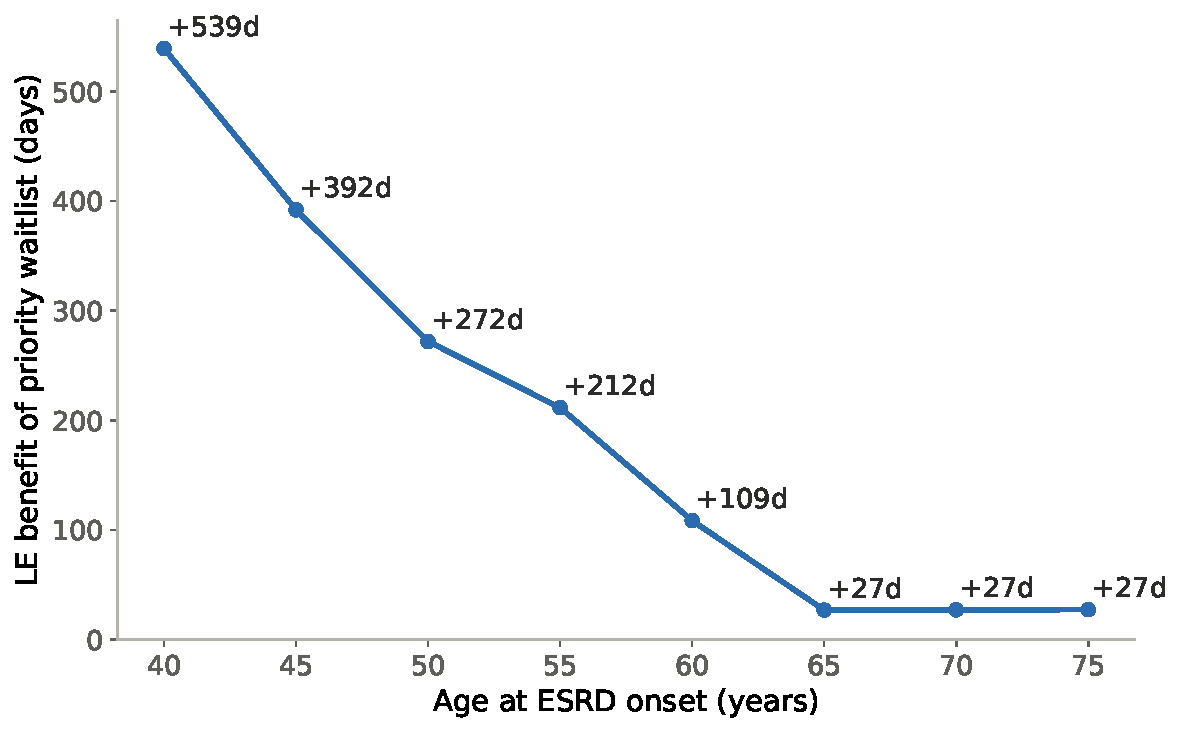
\includegraphics[width=\linewidth]{figures/esrd_conditional_age_sweep.pdf}
	\caption{\textbf{Priority waitlist LE benefit conditional on ESRD onset, by age.} $\Delta\text{LE}$ (priority minus standard waitlist, days) for individuals who have already developed ESRD, as a function of age at ESRD onset. Conditional on ESRD, priority access is highly valuable: $+539$~days at age~40 onset, $+109$~days at age~60. This large conditional benefit is diluted to under 1~day at the population level by the low ESRD incidence in non-donors ($\approx 0.04\%$/15~yr) and in donors ($\approx 0.3\%$/15~yr).}
	\label{fig:esrd_conditional}
\end{figure}
